\documentclass[12pt,a4paper,oneside,final]{book}
\newcommand{\TITLE}{EXAMPLE OF BACHELOR THESIS TITLE WITH LENGTH OF TWO LINES}
\newcommand{\AUTHOR}{Student Name}
\newcommand{\ADVISOR}{Prof. Thesis Advisorus, Advisor}
\newcommand{\COADVISOR}{George Coadvisoris, S.Si, M.Si, Co-Advisor}
\newcommand{\DATE}{February 2023}

\title{\TITLE}
\author{\AUTHOR}
\date{\DATE}

\usepackage{natbib}
\usepackage{graphicx}
\usepackage{subfig}
\usepackage{fancyhdr}
\usepackage{lastpage}
\usepackage{setspace}
\usepackage{textcase} 
\usepackage{hyperref}
\usepackage{titlesec}
\usepackage{rotating}
\usepackage{array}
\usepackage{booktabs}
\usepackage{mdwlist}
\usepackage{amsmath}
%\usepackage{algorithm}
\usepackage[noend]{algpseudocode}
\usepackage[top=1in,bottom=1in,left=1.5in,right=1in]{geometry}
\usepackage{tabularx} %for automation of column widths so that the table spans the width defined by textwidth and linewidth
\usepackage{indentfirst}
\usepackage[subfigure]{tocloft} 
\usepackage{textcomp}
\usepackage{mathptmx}
\usepackage{multirow}
\usepackage[T1]{fontenc}
\usepackage[none]{hyphenat}
\usepackage{pgfplots}
\usepackage{enumitem}
\usepackage{amssymb}
\usepackage{array}
\usepackage{doi}
\usepackage{algorithm,algorithmicx}
\usepackage{afterpage}
\usepackage{lscape}
\usepackage{url}
\usepackage{listings,lstautogobble}
\usepackage{color}
\usepackage{pifont}
\usepackage{adjustbox}
\usepackage{longtable}
\usepackage{ltablex}
\pgfplotsset{compat=newest}
\pagestyle{empty}
\sloppy

\setcounter{secnumdepth}{3}
\setcounter{tocdepth}{3}

% Configure global line spacing
	\renewcommand{\baselinestretch}{1.5} 
%\linespread{1.5}

% Configure chapter & section heading
\titleformat{\chapter}[display]
{\normalfont\bfseries \filcenter}{Chapter {\thechapter}}{12pt}{}
\titlespacing*{\chapter}{0in}{0in}{0.4in}

\titleformat{\section}
{\normalfont\bfseries}{\thesection}{12pt}{}
\titleformat{\subsection}
{\normalfont\bfseries}{\thesubsection}{12pt}{}
\titleformat{\subsubsection}
{\normalfont\normalsize\bfseries}{\thesubsubsection}{12pt}{}

% Configure header and footer style
\fancypagestyle{plain}{
  \fancyhf{}
  \fancyhead[L]{\footnotesize{\TITLE}}
  \fancyhead[R]{\footnotesize{Page {\thepage} of \pageref{LastPage}}}
  \fancyfoot[R]{\footnotesize{\AUTHOR}}
  \renewcommand{\headrulewidth}{0.5pt}
  \renewcommand{\footrulewidth}{0.5pt}
}

% Configure bibliography management
\bibliographystyle{sgu-harvard}
\setlength{\bibhang}{0in}
\pagestyle{plain}

%configure so TOC have dots for chapter, default no dots
\renewcommand\cftchapaftersnum{.}
\renewcommand\cftchapdotsep{\cftdotsep}
\renewcommand{\contentsname}{Table of Contents}
\renewcommand\bibname{REFERENCES}

%-------------------------------------------------------------------
% Document's content
%-------------------------------------------------------------------

\begin{document}
	%
\begin{titlepage}
\begin{center}

PROPOSAL OF THESIS
\begin{spacing}{2}
	\textbf{ \TITLE} \\[0.7in]
\end{spacing}

\begin{spacing}{1.5}
	By \\ \AUTHOR \\ 22251030 \\[0.5in]
	
	I propose to the Advisors and to the Committee Members a study of the afore mentioned topic to be carried out in partial fulfilment of the requirements for the

    MASTER'S DEGREE \\ in \\ MASTER OF INFORMATION TECHNOLOGY \\ FACULTY OF ENGINEERING AND INFORMATION TECHNOLOGY \\[0.7in]
\end{spacing}
	  
\vfill
\centering 
\includegraphics{images/sgu}  \\%[0.7in]
\vfill



\hfil
\begin{spacing}{1}
	SWISS GERMAN UNIVERSITY \\
    The Prominence Tower \\
    Jalan Jalur Sutera Barat No. 15, Alam Sutera \\
    Tangerang, Banten 15143 - Indonesia \\[0.5in]
    
    July 2023
\end{spacing}

\end{center}
\end{titlepage}


	%
\begin{titlepage}
\begin{center}

\begin{spacing}{2}
    PROPOSAL OF THESIS
	\textbf{ \TITLE} \\[0.7in]
\end{spacing}

\begin{spacing}{1.5}
	By \\ \AUTHOR \\ 22251030 \\[0.5in]

    MASTER'S DEGREE \\ in \\ MASTER OF INFORMATION TECHNOLOGY \\ FACULTY OF ENGINEERING AND INFORMATION TECHNOLOGY \\[0.7in]
\end{spacing}
	  
\vfill
\centering 
\includegraphics{images/sgu}  \\%[0.7in]
\vfill

\hfil
\begin{spacing}{1}
	SWISS GERMAN UNIVERSITY \\
    The Prominence Tower \\
    Jalan Jalur Sutera Barat No. 15, Alam Sutera \\
    Tangerang, Banten 15143 - Indonesia \\[0.5in]
    
    January 2023
\end{spacing}


\end{center}
\end{titlepage}


	%\newcommand{\signrule}{\rule{\linewidth}{0.2mm}}

\chapter*{STATEMENT BY THE AUTHOR}
\thispagestyle{fancy}
\addtocontents{toc}{~\hfill\textbf{Page}\par}
\addcontentsline{toc}{chapter}{STATEMENT BY THE AUTHOR}

I hereby declare that this submission is my own work and to the best of my knowledge, it contains no material previously published or written by another person, nor material which to a substantial extent has been accepted for the award of any other degree or diploma at any educational institution, except where due acknowledgement is made in the thesis.

\vspace{0.35in}

\begin{table}[ht!]    
  \begin{center}
    \begin{tabular}{ p{3.0in} p{0.3in} p{1.5in} }
      \AUTHOR & & \\
      \signrule & & \signrule \\
      Student & & \centering Date
    \end{tabular}
  \end{center}
\end{table}
Approved by:

\vspace{0.5in}

\begin{table}[ht!]    
  \begin{center}
    \begin{tabular}{ p{3.0in} p{0.3in} p{1.5in} }
      \ADVISOR & &  \\
      \signrule & & \signrule \\
      Thesis Advisor & & \centering Date
    \end{tabular}
  \end{center}
\end{table}

\vspace{0.5in}

\begin{table}[ht!]    
  \begin{center}
    \begin{tabular}{ p{3.0in} p{0.3in} p{1.5in} }
      \COADVISOR & & \\
      \signrule & & \signrule \\
      Thesis Co-Advisor & & \centering Date
    \end{tabular}
  \end{center}
\end{table}

\vspace{0.5in}

\begin{table}[ht!]    
  \begin{center}
    \begin{tabular}{ p{3.0in} p{0.3in} p{1.5in} }
      Dr. Irvan Setiadi Kartawiria, S.T.,M.Sc. & & \\
      \signrule & & \signrule \\
      Dean of Faculty of Engineering and Information Technology & & \centering Date
    \end{tabular}
  \end{center}
\end{table}
	%\chapter*{ABSTRACT}
\thispagestyle{fancy}
\addcontentsline{toc}{chapter}{ABSTRACT}

\begin{center}
  \TITLE \\[36pt]
  By \\ [12pt] \AUTHOR \\
  \ADVISOR, Advisor \\ \COADVISOR, Co-Advisor \\[0.3in]
  \text{SWISS GERMAN UNIVERSITY} \\[36pt]
  
\end{center}
Begin typing the abstract here, 1.5 spaced. The abstract must include the following components: purpose of the research, methodology, findings, and conclusion. The abstract must it is imperative to prioritize clarity, conciseness, accuracy, and a logical flow. Begin by succinctly summarizing the key objectives, methods, and findings of your research. Avoid jargon and overly technical language, opting instead for clear and accessible terminology. Ensure that your abstract accurately reflects the content of your thesis, avoiding any misleading statements. Review and revise your abstract meticulously, eliminating unnecessary details and maintaining a concise yet informative tone throughout. Lastly, In the abstract of your thesis, ensure utmost clarity in conveying the research's objectives and its overall significance. Begin by succinctly articulating the main goals of your study, outlining what you aimed to investigate, discover, or achieve. Subsequently, expound on the relevance and broader implications of your research in the respective field or context. Highlight how your findings contribute to existing knowledge, address gaps, or potentially impact practical applications. Keep the abstract concise, focusing on conveying essential information rather than delving into intricate details. 

\vfill

\noindent \emph{Keywords}: Keyword1, Keyword2, Keyword3, Keyword4, Keyword5 (use scientific terms).

	%
%\chapter*{Copyright}
\thispagestyle{fancy}

%\clearpage
\vspace*{\fill}
{\setstretch{1.0}
\begin{center}
		\textcopyright{} copyright 2023\\
		by Student Name\\
		All rights reserved
\end{center}
\vfill % equivalent to \vspace{\fill}
%\clearpage
	%
\chapter*{DEDICATION}
\thispagestyle{fancy}
\addcontentsline{toc}{chapter}{DEDICATION}
{\setstretch{1.5}
\begin{center}
	Dedication is normally short and direct. Example: I dedicate this works for the future of the country I loved: Indonesia
\end{center}

	%
\chapter*{ACKNOWLEDGEMENT}
\thispagestyle{fancy}
\addcontentsline{toc}{chapter}{ACKNOWLEDGEMENT} 
This is the part where you express your gratitude to all parties involved in the success of your thesis work. However, keep it simple and short. 
Example: I wish to thank the members of my committee for their support, patience and good humor. Their gentle but firm direction has been most appreciated. \ADVISOR was particularly helpful in guiding me toward a qualitative methodology. \COADVISOR interest in sense of competence was the impetus for my proposal. Finally, I would like to thank Dr. Stephen Fain. From the beginning, he had confidence in my abilities to not only complete a degree but to complete it with excellence.
I have found my coursework throughout the Curriculum and Instruction program to be stimulating and thoughtful, providing me with the tools with which to explore both past and present ideas and issues.



	\tableofcontents
	\addcontentsline{toc}{chapter}{TABLE OF CONTENTS}
	\cleardoublepage
	\listoffigures
	\addcontentsline{toc}{chapter}{LIST OF FIGURES}
	\cleardoublepage
	\listoftables
	\addcontentsline{toc}{chapter}{LIST OF TABLES}
	\cleardoublepage
	
  	\chapter{INTRODUCTION}
\label{chap:introduction}
\thispagestyle{fancy}
	
Special Note: Ensure that your thesis demonstrates a clear and realistic scope in terms of resources required, with a comprehensive contingency plan in place. Maintain a high level of clarity and coherence throughout the proposal by organizing the content logically and following a structured format. Pay meticulous attention to grammar, style, and language use, while also conducting thorough proofreading and editing to enhance the overall writing quality.

\section{Background}
\label{sec:background}
For your thesis introduction, keep it concise and clear. Start by explaining the background and why your research is important. State your research goal and mention the gap in existing knowledge. Present your thesis statement and mention any relevant concepts or theories, citing references as needed. Justify why your research problem matters and how it's novel. Ensure smooth transitions between ideas, maintain reader interest, and write in a well-structured and engaging manner, setting the stage for the rest of your work.

\begin{itemize}
	\item List 1
	\item List 2
	\item List 3
\end{itemize}

	\section{Problem Statement}
	\label{sec:problem-statement}
	In formulating a research problem, it is essential to identify a specific and well-defined issue within your field of study that warrants investigation. The research problem should be clear, concise, and compelling, posing a question or challenge that both contributes to the existing body of knowledge and has practical relevance. It should reflect a gap in current understanding, necessitating further exploration and analysis. A strong research problem serves as the foundation upon which your entire study is built, guiding the research process, and helping to define the scope and objectives of your research. To assist in defining research problems, a fishbone diagram is recommended.

	\begin{figure}[htbp]
		\centering 
		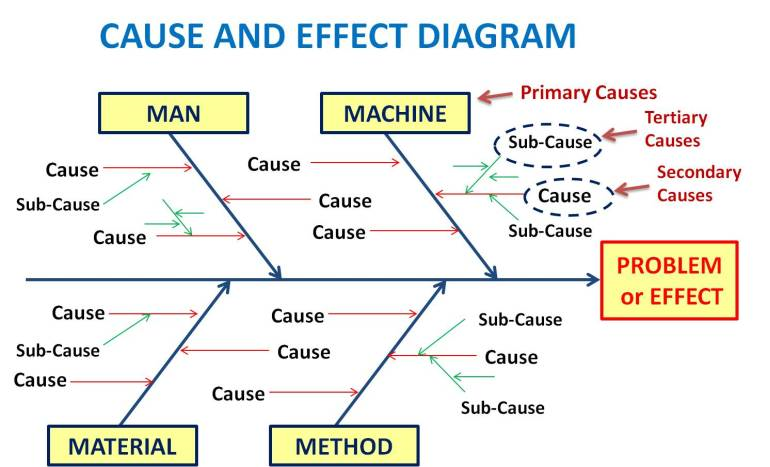
\includegraphics[width=0.8\textwidth]{images/fishbone.png}
		\caption{Example of fishbone diagram}
		\label{fig:fishbone}
	\end{figure} 

	Note: when you’re thinking about research problem and objective, please make sure your Feasibility, Realistic Timeline, Resource Availability, Data Availability, and Contingency Plan (Plan A, Plan B and Plan C with different scoping).

	\section{Research Objective}
	\label{sec:research-objective}	
	For Research Question and Objective, making sure they are specific and match the research problem. Ensure they can be measured and are feasible. Cover all aspects of the research objectives, problems, and gaps in a complete and coherent manner. Stay open to different approaches and maintain consistency throughout. Use clear and precise language while emphasizing the relevance and importance of your research. Keep in mind that each objective and question should be achievable within your research context. Overall, create a well-organized thesis that addresses each element of the assessment format effectively.
    
	\section{Research Question}
	\label{sec:research-question}
	For Research Question and Objective, making sure they are specific and match the research problem. Ensure they can be measured and are feasible. Cover all aspects of the research objectives, problems, and gaps in a complete and coherent manner. Stay open to different approaches and maintain consistency throughout. Use clear and precise language while emphasizing the relevance and importance of your research. Keep in mind that each objective and question should be achievable within your research context. Overall, create a well-organized thesis that addresses each element of the assessment format effectively.
    	
    \section{Hypothesis}
  	\label{sec:hypothesis}
		This is the body of your thesis. Please check that your body of thesis consistency in term of font type, font size, spacing, and margin are maintained. This is the body of your thesis. Please check that your body of thesis consistency in term of font type, font size, spacing, and margin are maintained.
	
	 \section{Research Scope and Limitation}
	  \label{sec:research-scope-of-works}
		This is the body of your thesis. Please check that your body of thesis consistency in term of font type, font size, spacing, and margin are maintained. This is the body of your thesis. Please check that your body of thesis consistency in term of font type, font size, spacing, and margin are maintained.

	\section{Significance of Study}
	\label{sec:significance-of-study}
	In this section you need to highlight or showcase the originality, methodological innovation, and practical implications for the field. Remember to emphasize the field relevance to the stakeholder, and the broader implications, while maintaining comprehensiveness and balance. Overall, your thesis should demonstrate how your work aligns with existing knowledge, contributes to theory and practice, and possesses the potential to reshape the field.

	\section{Thesis Structure}
	This is the body of your thesis. Please check that your body of thesis consistency in term of font type, font size, spacing, and margin are maintained. This is the body of your thesis. Please check that your body of thesis consistency in term of font type, font size, spacing, and margin are maintained.
    
  	
\chapter{LITERATURE REVIEW}
\label{chap:literature-review}
\thispagestyle{fancy}
(Sub-chapter mentioned below is for typing guidelines only. Discuss with your advisor for the actual sub-chapter title and content). It is advisable (not-compulsory) to write introductory sentences here prior to further elaboration in the sub-chapter. The sub-chapter mentioned here serves as samples, and should not be considered as compulsory. Contact your thesis adviser for the actual sub-chapter division.
	 
\section{Theoretical Perspectives}
\label{sec:theoretical-perspective}
This is the body of your thesis. Please check that your body of thesis consistency in term of font type, font size, spacing, and margin are maintained \cite{gdbusecaseneo4j}. This is the body of your thesis. Please check that your body of thesis consistency in term of font type, font size, spacing, and margin are maintained. This is the body of your thesis \cite{linuxstatistic}. Please check that your body of thesis consistency in term of font type, font size, spacing, and margin are maintained \cite{shin2022focusing}.

\begin{figure}[htbp]
	\centering 
	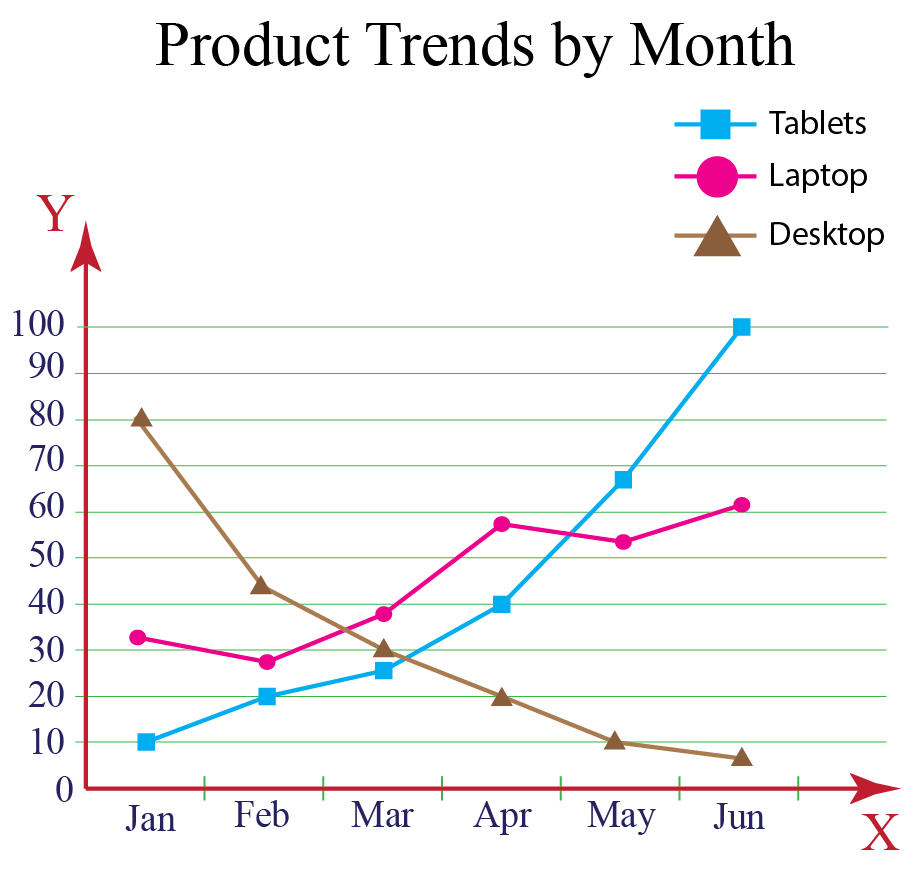
\includegraphics[width=0.6\textwidth]{images/graph.png}
	\caption{Another example of figure placement in your body of thesis and its label}
	\label{fig:figure-example}
\end{figure} 
 
Figure \ref{fig:figure-example} is ....

This is the body of your thesis. Please check that your body of thesis consistency in term of font type, font size, spacing, and margin are maintained \cite{djap_xb_pot}. This is the body of your thesis. Please check that your body of thesis consistency in term of font type, font size, spacing, and margin are maintained \cite{cabral2019review}. This is the body of your thesis \cite{boffa2022towards}. Please check that your body of thesis consistency in term of font type, font size, spacing, and margin are maintained \cite{exabeam}.This is the body of your thesis. Please check that your body of thesis consistency in term of font type, font size, spacing, and margin are maintained.This is the body of your thesis. Please check that your body of thesis consistency in term of font type, font size, spacing, and margin are maintained. This is the body of your thesis. Please check that your body of thesis consistency in term of font type, font size, spacing, and margin are maintained.

Please note that all figures and graphs in the body of thesis are in grayscale, unless really necessary. Color printed material can be placed as appendix. Cite it as  \ref{fig:figure-example}

\section{Previous Studies}
\label{sec:previous-studies}
I want to cite a paper from \cite{shrivastava2019attack}, because ... \\

This is the body of your thesis. Please check that your body of thesis consistency in term of font type \cite{honeypot_spitzner}, font size, spacing, and margin are maintained. This is the body of your thesis. Please check that your body of thesis consistency in term of font type \cite{noor2019machine}, font size, spacing, and margin are maintained.

\begin{table}
	\centering
	\caption{Example of Comparison Table}
	\begin{tabularx}{\linewidth}{X c X X}
			\hline
			\textbf{No} & \textbf{Paper} & \textbf{Description} \\ 
			\hline
			Feature number 1 & 1 & This is the description of what you want to explain, please elaborate in a clear and concise sentence & Sesuatu \\
			Feature number 2 & 2 & This is the description of what you want to explain, please elaborate in a clear and concise sentence & Sesuatu \\
			Feature number 3 & 3 & This is the description of what you want to explain, please elaborate in a clear and concise sentence \\
			Feature number 4 & 4 & This is the description of what you want to explain, please elaborate in a clear and concise sentence & Sesuatu \\
			\hline
	\end{tabularx}
	\label{tab:example-of-comparison-table}
\end{table}

This is the body of your thesis. Please check that your body of thesis consistency in term of font type, font size, spacing, and margin are maintained. This is the body of your thesis. Please check that your body of thesis consistency in term of font type, font size, spacing, and margin are maintained. This is the body of your thesis. Please check that your body of thesis consistency in term of font type, font size, spacing, and margin are maintained.

Please make sure that you use consistent style of table throughout your body of thesis. This is the body of your thesis. Please check that your body of thesis consistency in term of font type, font size, spacing, and margin are maintained. This is the body of your thesis. Please check that your body of thesis consistency in term of font type, font size, spacing, and margin are maintained.

  	\chapter{RESEARCH METHODS}

\begin{figure}[htbp]
	\centering 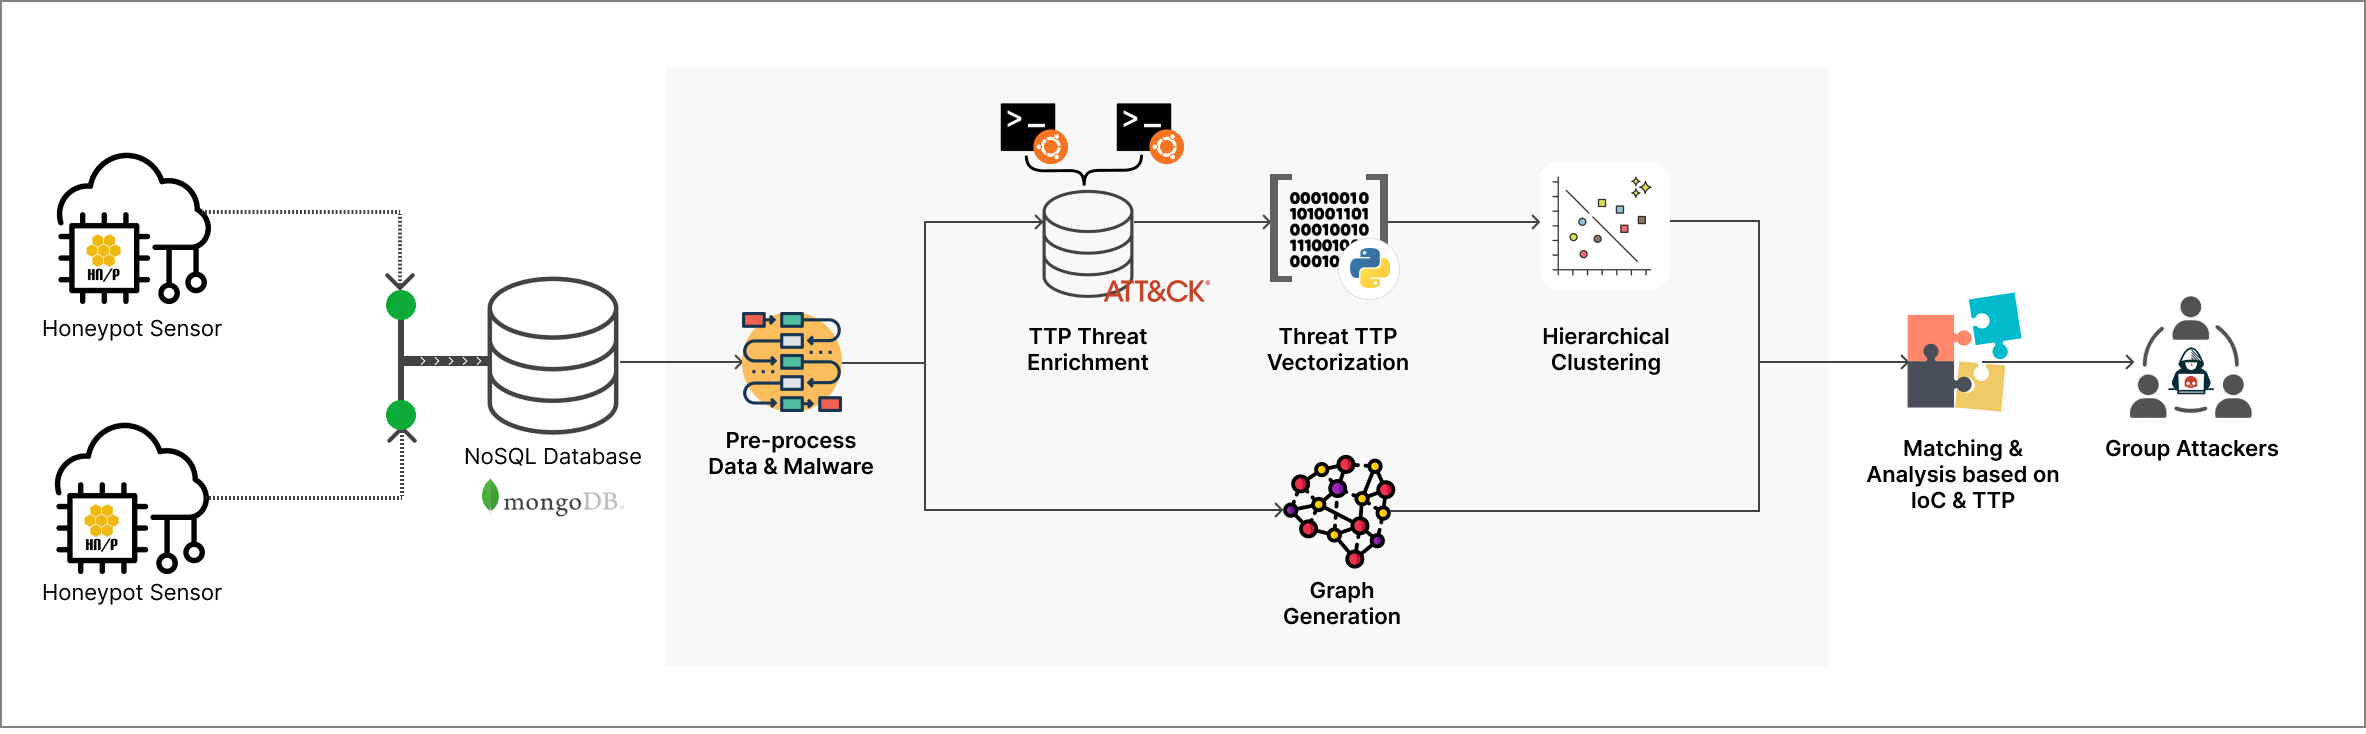
\includegraphics[width=1.0\textwidth]{images/framework.png}
	\caption{Research Framework}
	\label{fig:framework}
\end{figure} 

\section{Research Methodology}
The research methodology section of a thesis is pivotal in ensuring the credibility, validity, and replicability of the study. It serves as the blueprint for conducting the research, like doing literature review, and do some qualitative and/or quantitative methods, detailing how data will be gathered, sample selection, data analysis techniques, and strategies for addressing potential biases. Figure \ref{fig:framework} show the research framework of this research

\section{Research Framework}
A well-crafted research framework serves as the foundational blueprint for any scholarly investigation, providing a clear and structured pathway for the research process. It is essential to begin with a concise and focused thesis statement that articulates the research problem and its significance. Subsequently, the framework should delineate the research objectives, defining what the study aims to achieve. A thorough literature review should be integrated to establish the theoretical and empirical context, identifying gaps and opportunities for contribution. Methodological choices and data collection techniques must be explicitly outlined, ensuring the study's validity and reliability. It’s important the proposed framework includes how to evaluate and validate the research results. A well-structured research framework not only guides the researcher but also enhances the rigor and credibility of the study, ultimately contributing to the advancement of knowledge in the chosen field. Example using STRIDE for Threat Modelling, using NIST SP 800-37 Rev. 2 for Risk Management Framework and many more. 
  	%\chapter{RESEARCH METHODS}
(Sub-chapter mentioned below is for typing guidelines only. Discuss with your advisor for the actual sub-chapter title and content).It is advisable (not-compulsory) to write introductory sentences here prior to further elaboration in the sub-chapter. The sub-chapter mentioned here serves as samples, and should not be considered as compulsory. Contact your thesis adviser for the actual sub-chapter division.

\section{Initial Evaluation}
This is the body of your thesis. Please check that your body of thesis consistency in term of font type, font size, spacing, and margin are maintained. This is the body of your thesis. Please check that your body of thesis consistency in term of font type, font size, spacing, and margin are maintained. This is the body of your thesis. Please check that your body of thesis consistency in term of font type, font size, spacing, and margin are maintained.

\section{Data Analysis}
This is the body of your thesis. Please check that your body of thesis consistency in term of font type, font size, spacing, and margin are maintained. This is the body of your thesis. Please check that your body of thesis consistency in term of font type, font size, spacing, and margin are maintained. This is the body of your thesis. Please check that your body of thesis consistency in term of font type, font size, spacing, and margin are maintained.

\begin{table}
	\centering
	\caption{Example of Comparison Table}
	\begin{tabularx}{\linewidth}{X c X}
			\hline
			\textbf{No} & \textbf{Paper} & \textbf{Description} \\ 
			\hline
			Feature number 1 & 1 & This is the description of what you want to explain, please elaborate in a clear and concise sentence \\
			Feature number 2 & 2 & This is the description of what you want to explain, please elaborate in a clear and concise sentence \\
			Feature number 3 & 3 & This is the description of what you want to explain, please elaborate in a clear and concise sentence \\
			\hline
	\end{tabularx}
	\label{tab:data-analysis-table}
\end{table}

This is the body of your thesis. Please check that your body of thesis consistency in term of font type, font size, spacing, and margin are maintained. This is the body of your thesis. Please check that your body of thesis consistency in term of font type, font size, spacing, and margin are maintained. This is the body of your thesis. Please check that your body of thesis consistency in term of font type, font size, spacing, and margin are maintained.

This is the body of your thesis. Please check that your body of thesis consistency in term of font type, font size, spacing, and margin are maintained. This is the body of your thesis. Please check that your body of thesis consistency in term of font type, font size, spacing, and margin are maintained. This is the body of your thesis. Please check that your body of thesis consistency in term of font type, font size, spacing, and margin are maintained.

  	%\chapter{CONCLUSION AND RECOMMENDATIONS}
(Sub-chapter mentioned below is for typing guidelines only. Discuss with your advisor for the actual sub-chapter title and content).It is advisable (not-compulsory) to write introductory sentences here prior to further elaboration in the sub-chapter. The sub-chapter mentioned here serves as samples, and should not be considered as compulsory. Contact your thesis adviser for the actual sub-chapter division.

\section{Conclusion}
This is the body of your thesis. Please check that your body of thesis consistency in term of font type, font size, spacing, and margin are maintained. This is the body of your thesis. Please check that your body of thesis consistency in term of font type, font size, spacing, and margin are maintained. This is the body of your thesis. Please check that your body of thesis consistency in term of font type, font size, spacing, and margin are maintained.

\section{Recommendations}
This is the body of your thesis. Please check that your body of thesis consistency in term of font type, font size, spacing, and margin are maintained. This is the body of your thesis. Please check that your body of thesis consistency in term of font type, font size, spacing, and margin are maintained. This is the body of your thesis. Please check that your body of thesis consistency in term of font type, font size, spacing, and margin are maintained.

  	
  \appendix
	\titleformat{\chapter}[display]
		{\normalfont\bfseries \filcenter}{Appendix{\thechapter}}{0.1in}{}[]
  	\chapter{Diagram}
\label{ap:sample-fingerprint-images}
\thispagestyle{fancy}

\begin{figure}
  \centering 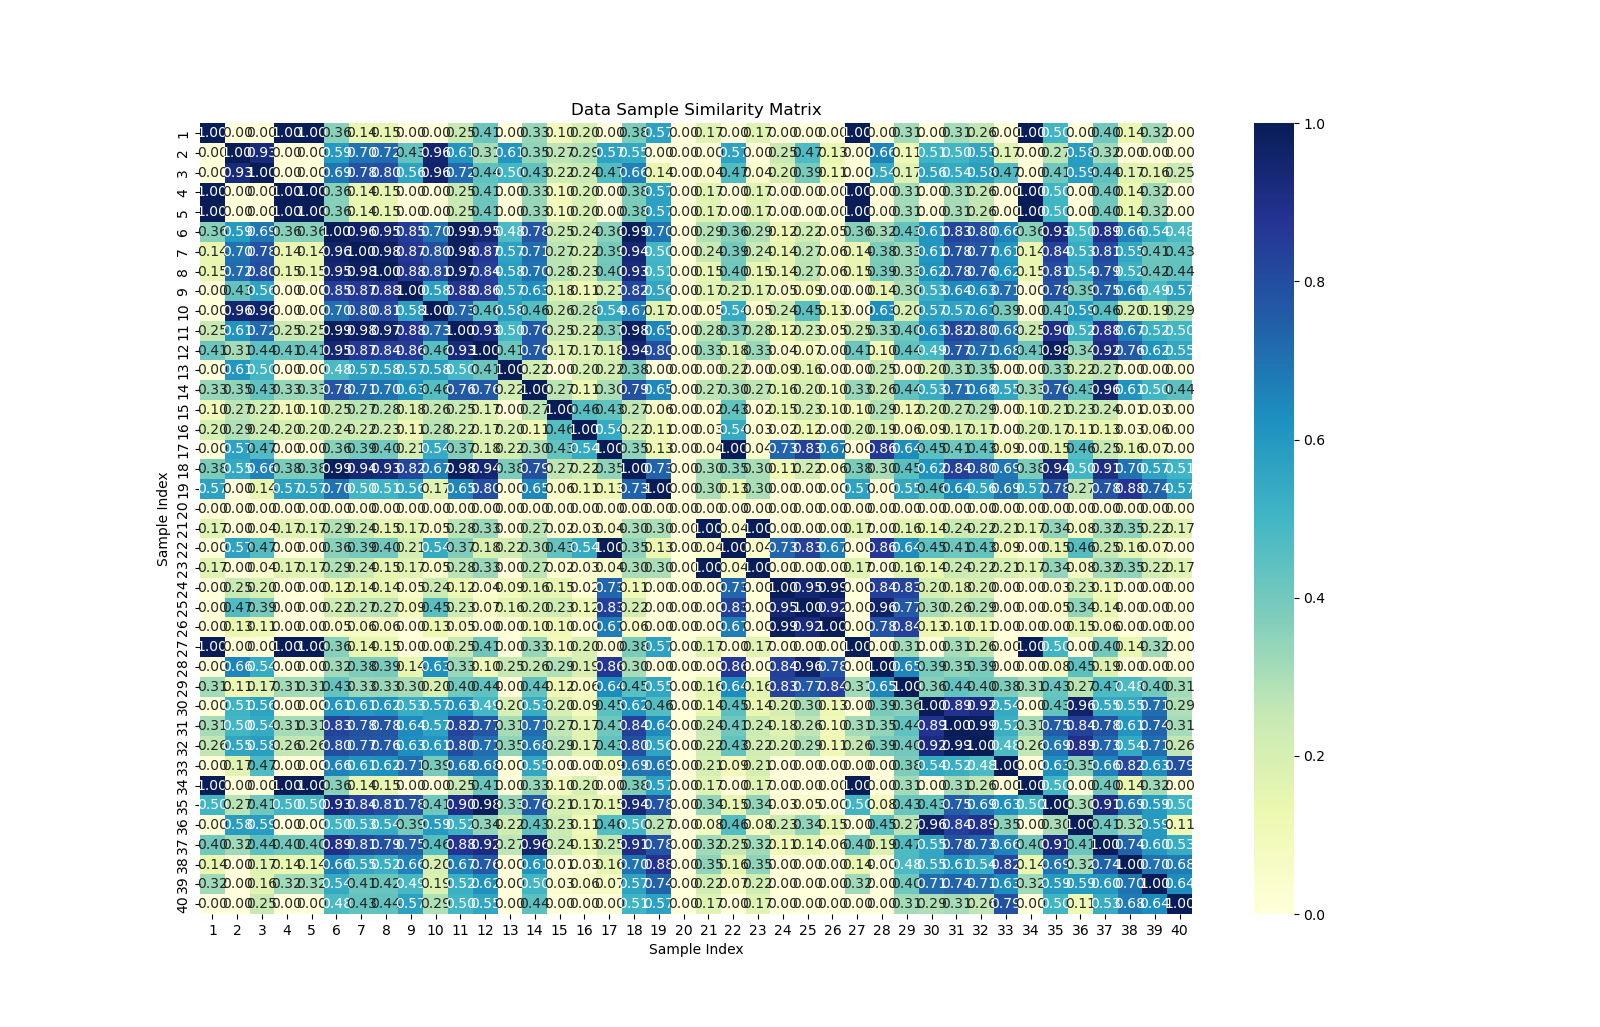
\includegraphics[width=\textwidth]{appendix/confusion_matrix_p2.png}
  \caption{Early Stage of Confusion Matrix}
  \label{fig:early-stage-of-confusion-matrix}
\end{figure}

  	%\include{OtherAppendix}

  	\bibliography{MyBibliography}
  	\addcontentsline{toc}{chapter}{REFERENCES}

\end{document}
